
\section{Motivation}
	%BaseliyosJacob
	%additions / changes by JakobGärtner
The openETCS work package 3 (WP3) aims to provide – amongst others - the software architecture for the openETCS kernel in order to eventually build the software itself. 

The WP3  partners had by the end of 2014 put great effort in the openETCS software design, thus far without making definite choices on the software architecture itself respective of functional breakdown and data structures of the openETCS kernel. Since the project planning foresees in the production of a reference software to be used as a demonstrator by June 2015, it was of paramount importance that a first design delivarable of the openETCS kernel architecture be finalized shortly but no later than November 2014.

This document shows a snapshot of the software and will also give an outlook to the scope of the next iteration and the final objectives.


\section{Objectives}
%Baseliyos Jacob
The prime objective of WP3 is to produce a fully formal prototype for the openETCS reference system that can function as a demonstrator in collaboration with WP 4 and WP 5  for the openETCS approach and will be used as such in the final phase of the project. That phase is the first half of 2015.  This objective is defined as … 

High level Objectives of this work:
<<any further general statements on the ITEA2  objectives, like…>>

\begin{itemize}
\item Work on a model bases approach and process for effective collaborative work within an international ETCS developer team as stated above, the project needs a definite architecture design by the end of 2014.

This document targets:
\item Defining the general design and conditions of the openETCS architecture, functional breakdown, data structures, behaviour and interfaces.
\item Providing the guidelines for discussion during the workshops that are planned in October and November 2014 that will result in the final and decisive version of this document
\item Being the ‘platform’ for finalization i.e. whatever be the products or results of the workshops shall be integrated in this document.
\end{itemize}

Apart from these general objectives, the document means to provide for the materials that will enable WP3 partners to improve the efficiency of the Work Package activities:
\begin{itemize}
\item The comprehensive architecture design shall enable splitting the work load according to the building blocks defined by the architecture and allocate strictly compartmented work parcels or activities to WP3 partners.
\item Doing so will enable WP3 to avoid any double work
\item  Compartmenting the work load according to the functional building blocks as defined by the architecture will enable efficient planning of activities, be it individually or the integrated WP3 planning for the coming period, aiming at a just in time delivery of all results and products
\item  Compartment the work load according to the functional building blocks as defined by the architecture will enable efficient planning of activities, be it individually or the integrated WP3 planning for the coming period, aiming at a just in time delivery of all results and products
\end{itemize}

%\tbc
%JakobGärtner


\subsection{Scope of deliverables}

The primary objective of WP3 was to produce a rapid prototype for the openETCS reference system that can function as a demonstrator in collaboration with WP 4 and WP 5  for the openETCS approach and will be used as such in the final phase of the project. That phase is the first half of 2015.

We have to see this original objective in the context of the overall innovation promise of openETCS and the related exploitation potential.
Taking into account the current situation of the project (as of Nov. 2014) we have to make choices that make sure that the remaining budget and resources are wisely used, which necessitates that the WP3 deliverables become more "multi- purpose":

\begin{itemize}
\item provide a functional formal specification of openETCS, based on functional analysis, and traceable to the SRS.
 
\item Iteratively develop the software architecture and design description document (ADD) while using the formal specification as an executable functional model.
 
\item Utilise real- world use-case scenarios as early as possible in the development process.
\end{itemize}
 
If we take this approach, we can use the iterative development method, while applying a pragmatic view of SCRUM (which has been defined as the high- level project management method for this project) in order to build the following deliverables:

\begin{itemize}
\item An ADD document, providing a functional description of software architecture and design.
 
\item A RFC (Request For Comment) process that provides a cross- reference to the SRS, listing all requirements and design conflicts that have been identified during our work.
 
\item A formal, executable model of the openETCS kernel, which can directly be used as entry point into a (future) EN5012x SIL4 compliant software design process, as well as functional reference during simulation and on the planned WP5 demonstrator.
\end{itemize}
 
\begin{figure}
\centering
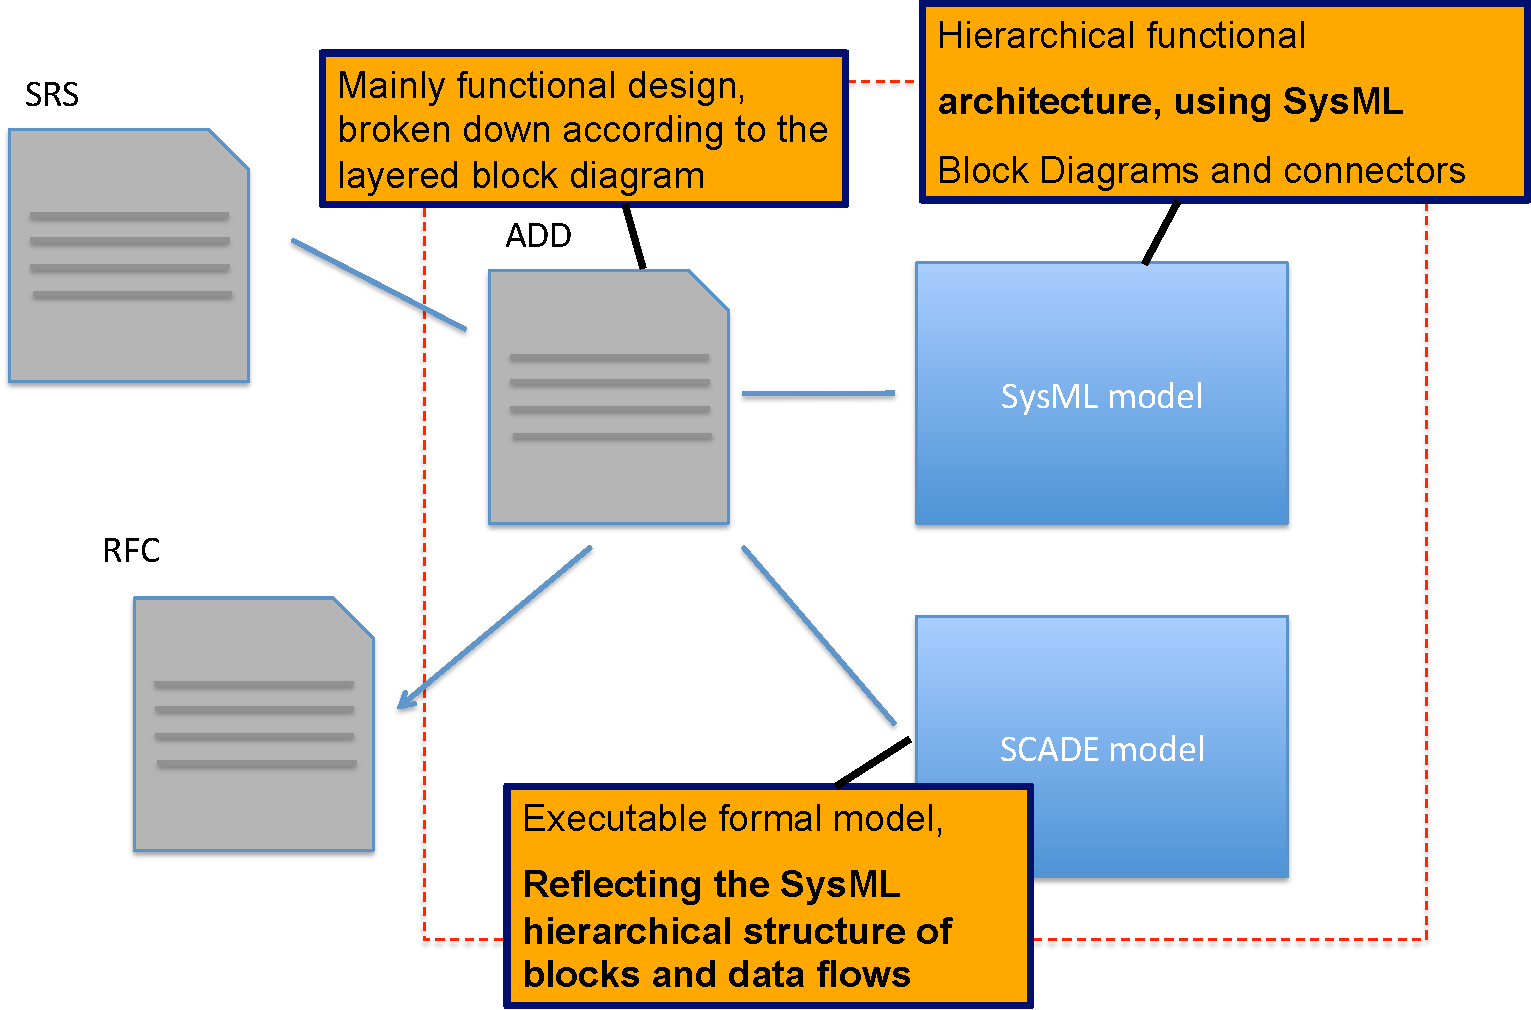
\includegraphics[width=\textwidth]{document-relations.pdf}
\caption{Document relationships in WP3.}
\label{fig:doc-rels}
\end{figure}

Each main WP3 collateral has it's distinct role in the overall project structure. For a schematic view of the dependencies, see Figure~\ref{fig:doc-rels}.


\subsection{Scope of the ADD document}
 
The ADD document is intended to provide the following main information:

\begin{itemize}
\item Internal guidance for the project: Provide authoritative guidance on process, responsibilties, process and workflow.
 
\item Architectural design description: Provide complete information on the overall architecture of the openETCS kernel functions.

\item Functional design description: Provide comprehensive information on the design of the system, which includes QoS aspects, interfaces, data types, algorithms and finally the full software design.
\end{itemize}

The nature of the development process implies that this document will be a "living document", meaning that it will be constantly updated, with new iterations being planned as follows:

\begin{itemize}
\item Intermediate work iterations (0.x): as required until the ITEA2 intermediate review (March 2015)

\item First main release (1.0): as a deliverable for the ITEA2 intermediate review (March 2015).

\item Intermediate work iterations (1.x): as required until the demonstrator milestone (June 2015).

\item Second main release (2.0): for the demonstrator milestone (June 2015).

\item Intermediate work iterations (2.x) for the rest of the project duration (until Oct 2015).

\item Final release (3.0) for the final review.
\end{itemize}

Intermediate work iteration shall be managed using the normal day-to-day pull/ review process, while main releases require a formal document sign-off.



\subsection{Scope of the User Validation Scenarios}

The work of WP3 has now been aligned to the milestones that are relevant for the overall project:
\begin{enumerate}
\item ITEA2 intermediate review (March 2015)
\item Demonstrator milestone (June 2015)
\item Final review (End of 2015)
\end{enumerate}

In order to support the functional approach, we use operational scenarios that are described the the User Validation Scenario Document.

These are based on the following data:
\begin{itemize}
\item Rules from NS for the operation of trains
\item Infrastructure data from the Utrecht- Amsterdam line
\end{itemize}

In order to support the functional analysis, which is aligned with the project's milestones, this document will define use cases along the following principles:

\begin{enumerate}
\item Selected operational scenarios on selected sections of the Utrecht- Amsterdam track

Based on nominal scenarios, our simulated train will drive across actual (simulated) infrastructure, selecting only a few, typical balise groups.
This will allow WP3 to implement the relevant mode/level/message (balise and RBC) functionality first.

The openETCS kernel model has been complemented by a simple DMI representation, in order to validate actual behaviour. 

In march 2015, only basic scenarios will be demonstrated, which have been organised as use cases, based on a plant/ controller co-simulation concept.

The future 


\item Selected operational scenarios on the full Utrecht- Amsterdam track

Based on nominal scenarios, our simulated train will drive across actual (simulated) infrastructure, covering the entire Utrecht- Amsterdam track.
This will allow WP3 to implement the relevant mode/level/message (balise and RBC) functionality first, fo full functional coverage of the test track.

Compared to the fist step in March, we will also cover more operational scenarios according to the NS operational rules.

A generic, interactive simulation concept will be created for this purpose. 

The entire track with its 488 balise groups and known (real) RBC messages as well as specific validation scenarios will be modelled.

A presentation of this concept can be found in the section "Dynamic Simulation".

\item Full coverage of Utrecht- Amsterdam

For the final review, we will prepare a openETCS kernel software that can run defined scenarios, accordiing to the NS operation regulation, across the entire Utrecht- Amsterdam line, either replaying actual train rides or simulating various events, nominal and non- nominal.

In cooperation with WP4 and WP5 this will provide additional input for demonstration and validation.
\end{enumerate}



\subsection{Scope of the RFC process}

The RFC document is a deliverable that was added to the WP3 set of documents during the Nov 3-7, 2014 Munich workshop.

Most (industrial) ETCS OBU systems have been built based on pure SRS analysis. at least in theory. In practise, each implementation is derived from the SRS, but with a mindset that is partially driven by the company culture and local operational regulation prior to ERTMS introduction.

This has lead to a plethora of ETCS systems, which exhibit subtle differences which lead to incomplete compatibility between OBUs and track equipment of different suppliers. Each OBU works best on a track which was built by the same supplier in the same country.

One of the objectives of openETCS is to provide a reference design for an ETCS UBU that reduces these variations.

The experts of WP3 and WP4 agree that a functional approach will lead to a better understanding of the system. As the SRS remains the formal reference, we have to provide formal feedback which is traceable to the SRS.

This is the objective of the RFC document.

The RFC document shall be structured following the paragraphs in the SRS and shall provide full traceability to the openETCS ADD.
Each design decision that can be traced to a deviation from the SRS or that highlights inconsistencies inside the SRS shall be documented in the RFC.

The RFC is hence a deliverable that provides formal feedback to the relevant ERTMS stakeholders.

(we still have to discuss the precise interaction between the SRS Analysis effort, WP4 and this RFC document)

The nature of the development process implies that this document will be a "living document", meaning that it will be constantly updated, with new iterations being planned as follows:

\begin{itemize}
\item Intermediate work iterations (0.x): as required until the ITEA2 intermediate review (March 2015)

\item First main release (1.0): as a deliverable for the ITEA2 intermediate review (March 2015)

\item Intermediate work iterations (1.x): as required until the demonstrator milestone (June 2015)

\item Second main release (2.0): for the demonstrator milestone (June 2015)

\item Intermediate work iterations (2.x) for the rest of the project duration (until Oct 2015)

\item  Final release (3.0) for the final review.
\end{itemize}

Intermediate work iteration shall be managed using the normal day-to-day pull/ review process, while main releases require a formal document sign-off.


\subsection{Objectives and scope related to formal executable model}

During the previous iterations of this document, it was proposed to use a traditional waterfall model in order to define the architecture and subsequently the functional and software design of the openETCS kernel software. We have now shifted the design paradigm to a more agile process, where we will use iterations (functional analysis, implementation of prototype formal executable model, refinement) in order to design the software modules. (bottom- up design of modules)

These will then be merged into a top- down architecture by the chief architect, using best practises that are well established for data- flow oriented software designs.

The result will be a functional, formal model, from which code can be generated that implements the functionality fin an hardware- independent way.

This code is hardware- and platform agnostic and can be integrated with the openETCS runtime environment, which is adaptable to different system architectures and APIs.




\section{Roles, responsibilities and tasks}
%\tbc
%Baseliyos Jacob
In this section, the roles and responsibilities of the WP3 partners are confirmed, especially where they divert from what has been agreed upon at the start of WP3:
\begin{itemize}
\item\textbf{Responsibilities} First of all, in the last WP 3 meeting in Brussels on  10.09.2014 DB proposed to take over the lead of the architecture design and functional breakdown. At the subsequent weekly scrum meeting on 12.09.2014,  it was agreed upon by all participants that DB will take over the lead (see Appendix … );\\
\item\textbf{Planning:} Alstom as WP 3 leader will remain to be responsible for the planning and the allocation of the defined tasks to the different partners\\
\item\textbf{Roles:} Alstom will also coordinate the work and safeguard that the defined results will be delivered according to the quality requirements that are agreed within the ITEA2 project and the schedule and the milestones that will be agreed upon during the coming workshops;\\
\item All WP3 partners will deliver the results or products according to planning as will be agreed upon during the said workshops. \\

In the interest of a swift production of the critical documentation of which this version is a draft, specific tasks will be defined in terms of concrete results to be delivered, the timeframes in which these results must be produced and the partner who shall be responsible for that specific result and the planning. This is to safeguard the timely delivery. The process will be described in the next sections.
\end{itemize}



%\tbc
%JakobGärtner for the chapter on openETCS design process



\section{openETCS Design Process}


\subsection{SRS- Driven Approach vs. Functional Approach}

Most attempts to formalise the ETCS onboard software have been focusing on creating models that were directly mirroring the SRS specification.
While this gives a full picture of the status quo of the SRS, it is not sufficient in order to fully understand the main issues that stem from the approach by which the SRS was conceived.

The SRS is aiming in what could be called the quadrature of the circle:
\begin{itemize}
\item Define a common specification of all aspects of the requirements of the ETCS system (Basic System Description, Principles, Functionality, Procedures and Application Level Communication Protocols, amongst others)
\item Create a framework that is compatible with all the local ways of driving trains
\item Ensure a framework for simple interoperability 
\item Give a full understanding of the wayside and onboard views of the system
\end {itemize}

Instead of building yet another copy-paste direct formalisation of the ETCS SRS, we are proposing a different approach:
\begin{itemize}
\item Functional analysis of the SRS
\begin{itemize}
  \item onboard point-of view
  \item SRS driven
  \item  Focused on the reference track (ETCS L2 Utrecht- Amsterdam)
\end{itemize}
\item Formalisation
\begin{itemize}
  \item Executable formal model (using SCADE tool suite)
  \item Dynamic simulation 
\end{itemize}
\item Validation
\begin{itemize}
  \item interface to WP4
\end{itemize}
\end{itemize}

Together with the document structure described above, this will for the first time lead to a OBU- centric formalisation of the SRS, with systematic Change Request process (through our RFC approach) and a functional reference that can be used to validate ETCS OBU software as well as wayside implementations once it is completed.

\subsection{Top- down vs. Bottom- Up}

The functional approach, together with other considerations mandated a combined top-down and bottom up design approach.
While the basic architecture was derived from existing architectures, with basic concepts and functional breakdown derived from the existing implementations of the WP3 leader, the actual functional analysis and the related software design was built bottom-up.

Thanks to the model- based formal design approach, the components could then be seamlessly merged with the top-down architecture.

Using this approach, the system and software architecture was at a relatively immature approach when we split the work in order to separately analyse and design the different functional blocks of the system.

The openETCS agile approach allows to iteratively integrate and align the top-down architectural view with the separately developed main functional blocks.


\subsection{Working groups}

While the basic architectural concept has been driven jointly by Alstom, DB and NS, the analysis and design of the functional blocks was distributed into working groups. Each working group consists of a combination of application/ analysis specialists and software/SCADE specialists.

\subsection{Use- case driven setting of priorities}

In order to focalise the work and to ensure our functional approach, DB has taken the role of product owner. 
As a reminder: in an agile/ SCRUM project management approach, the product owner has the responsibility to represent the interests of the customer.
The goal being to prove the openETCS concept and model on the ETCS L2 Utrecht- Amsterdam line, DB is formulating a set of at first very basic, then advanced and towards project completion comprehensive and complete scenarios and requirements for demonstration.

In- line with agile project management methodology, these requirements are presented to the WP3 team in the form of "user stories" which help to drive the project priorities.

\subsection{integration}

Integration on openETCS context is focusing on several aspects:
\begin{itemize}

\item Integration of SCADE functional blocks with overall SCADE architectural model

In a SCADE context, model-to-model integration is straightforward. As each functional block has a clear interface and all blocks have identical semantics we could follow an iterative, constructive and agile approach.
Integration was mainly driven by alignment of interfaces and validated by interactive simulation. 


\item Integration of openETCS model with WP3 simulation environment 

For the March 2015 ITEA review, a simple dynamic simulation environment was set up using SCADE tools (SCADE Display to build a first version of an openETCS DMI software, SCADE Rapid Prototyper to interact with the simulator).
Integration of the openETCS OBU software model followed the same principles as model-to-model integration.
The same concept will be extended for a full dynamic simulation of the Utrecht-Amsterdam line in interaction with the openETCS reference model.


\item Integration of openETCS model with openETCS runtime

Currently, the demonstration is purely on model/ simulation level. However, since the openETCS toolchain allows for automatic code generation, we will integrate the generated code with the openETCS runtime. 
As the generated code is strictly target agnostic, integration can be adapted very flexibly to different hosts and execution models.
Details of this integration phase will be discussed in the final version of this document, a first overview is given in the section discussing the APIs.
%
%
%\item Integration on EVC/ openETCS OBU
%
%The actual hardware integration 
%  ---------(this item is deferred for now// Jakob)
%
\end{itemize}

\subsection{Towards EN50128 SIL4 objectives, interface to WP4}

One of the objectives of openETCS is to demonstrate feasibility of the approach and concept in a CENELEC context.
While we are focusing on analysis and design for now, we will also formulate a certification strategy.

An actual EN50128 certification of the openETCS software is beyond the scope of this project.


%
% The following section commented out.
%
%REASON: this is/was an internal directive 


%\section{Assumptions and preconditions}
%\tbc
%Baseliyos Jacob
%\begin{itemize}
%\item All future contributions shall be fully aligned an compliant the finalised and approved document 
%\item Alls documents produced by the partners are requested to be compliant and merge to this document; other contributions will be discarded
%\textbf{The workshops are all about working as swift, as efficient and as productive as possible and make full use of the potential made available for these workshops by the partners. It is expected that the partners in the workshops will have the express intention to:}
%\item Contribute to the workshops with the intention to finalise the openETCS architecture;\\
%\item Provide resources according to the agreements made prior to the Workshops;\\
%\item Focus primarily on  getting concrete results regardless of methodological issues that might arise. Where necessary or opportune, classical project management methodology will be applied;\\
%\item Provide full transparency with respect to experience, knowledge base and information touching the subjects to be treated in the workshops;\\
%\item Document on paper or electronically all output of the workshops and integrate these with the underlying document;\\
%\item Restrict discussions only to topics that have an immediate impact on the content or the quality of the end product: the improved version of this document.\\
%\end{itemize}

\section{openETCS history and iterations}
%\tbc
%BaseliyosJacob
The openETCS Architecture and Design is being implemented in iterations. The current step (third iteration) is implementing essential kernel functions of the ETCS system. 
For a better understanding of the scope the Iteration is described in the following.

Third Iteration Functional Scope: The OBU functions for Szenarios defined in chapter 3.

The openETCS third iteration model is defining the architecture and design of the openETCS OBU software. 
It is referencing  \cite{subset-026} UNISIG Subset\_026 version\_3.3.0. 

The appropriate functionality has been divided into a number of functional blocks that are being analysed and designed by work groups (as described in the previous section of this document).

The third iteration of the openETCS modelling effort is focusing on demonstrating some simple scenarios on the actual (for now simulated) Utrecht- Amsterdam infrastructure.
